%!TEX ROOT=formularioMatematica.tex

\section{Integrali}
\subsection{Integrali indefiniti}
Sia $f$ una funzione continua in $[{a,b}]$. Allora $f'(x)$ è la sua derivata, $F(x)$ è una primitiva.
Bisogna quindi definire una primitiva di una funzione
\begin{primitiva}
  Una funzione $F(x)$ si dice primitiva della funzione $f(x)$ continua in $[{a,b}]$ se
  \begin{equation*}
    F'(x) = f(x)
  \end{equation*}
\end{primitiva}
Sia ad esempio $f(x) = \cos x$, $F(x)$ sarà allora quella funzione la cui derivata è $f(x)$. Quindi
$F(x)=\sin x$. Ma è soltanto questa? No, infatti anche $\sin x +1$ o $\sin x -\frac{e}{4}$ o 
qualsiasi altra funzione che abbia una costante. Così possiamo definire un insieme denominato
\textbf{totalità delle primitive} che le raccoglie tutte. L'operatore che permette di trovare questo
insieme è \textbf{l'integrale indefinito}
\begin{equation*}
  \int f(x)\,\dif x = \{F(x)+c\}
\end{equation*}
Scrivere $\dif x$ è necessario perché, come nella scrittura di Leibniz per le derivate, indica per
quale lettera si deve integrare.

\subsubsection{Differenziale}
Nella scrittura dell'integrale
\begin{equation*}
  \int f(x)\,\dif x
\end{equation*}
vediamo un termine $\dif x$ che non appartiene alla funzione. Quel termine prende il nome di 
\textbf{differenziale}. Osserviamo il significato geometrico.\\
Innanzitutto perché una funzione possieda differenziale, deve essere derivabile in $x_0$. Prendiamo
ad esempio un grafico
\begin{center}
  \begin{tikzpicture}[spy using outlines={circle, magnification=2, connect spies}]
    \tkzInit[xmin=-1,ymin=-1,xmax=4,ymax=4]
    \tkzGrid
    \tkzAxeXY
    \draw[name path=t,domain=-1:4,blue,thick] plot(\x,\x);
    \draw[name path=f,domain=0.1:4,red,thick,samples=500] plot(\x,{ln(\x)+1});
    \fill[olive, name intersections={of=t and f, total=\t}]
      \foreach \s in {1,...,\t}{(intersection-\s) coordinate (P) circle (2pt) node[below] {$P$}};
    \coordinate (H) at (2,0.92);
    \coordinate (Q) at (2,{ln(2)+1});
    \draw[name path=q, domain=2:2,magenta,dashed,thick] (2,1) -- ++(0,1.1);
    \fill[olive] (H) circle (2pt) node[below right]{$H$};
    \fill[olive] (Q) circle (2pt) node[right]{$Q$};
    \fill[olive, name intersections={of=t and q, total=\t}]
      \foreach \s in {1,...,\t}{(intersection-\s) coordinate (L)circle(2pt) node[above left]{$L$}};
    \draw[dashed, olive, thick] (P) -- (H);
    \filldraw[orange,fill opacity = 0.3] (P) -- (H) -- (Q) -- cycle;

    \coordinate (spypoint) at (6,1);
    \spy [blue, size=2.5cm] on ($(Q)!0.5!(L)$) in node[fill=white] at (spypoint);
\end{tikzpicture}
\end{center}
Come vediamo dalla figura, possiamo definire un punto $P(x_0,f(x_0))$ appartenente a $f(x)$ e
un altro punto $Q(x_0+\Delta x, f(x_0+\Delta x))$ appartenente sempre alla curva. $L$ invece si 
trova nell'intersezione tra il prolungamento di $\overline{HQ}$ e la tangente in $x_0$ alla curva.
$\overline{LH}$ viene definito il \textbf{differenziale} di $f$. Ma a quanto equivale? Se proviamo
a trovare l'angolo che la tangente fa con l'asse delle $X$
\begin{equation*}
  \tan \alpha = \frac{\overline{LH}}{\overline{PH}} = \frac{\dif f}{\Delta x}
\end{equation*}
dove $\dif f$ è il nostro differenziale. Ma l'angolo della tangente è equivalente al coefficiente
angolare, quindi alla derivata calcolata nel punto. Quindi
\begin{equation*}
  f'(x_0) = \frac{\dif f}{\Delta x}
\end{equation*}
da cui ne deriva che
\begin{equation*}
  \dif f = f'(x_0)\Delta x
\end{equation*}
Se ora immaginiamo di avvicinare il punto $Q$ sempre di più al punto $P$, come si farebbe per la
derivata, si nota che $\overline{LQ}\to0$. Quindi $\dif f\approx\Delta f$.\\
Prendiamo ora come esempio la funzione identica $f(x)=x$. Qual è il suo differeniziale?
\begin{equation*}
  \dif f(x) = \dif x
\end{equation*}
Quindi possiamo anche dire che
\begin{equation*}
  \dif x \approx \Delta x
\end{equation*}
Di conseguenza riscrivendo il differenziale
\begin{equation*}
  \dif f(x) = f'(x)\dif x
\end{equation*}

\subsubsection{Proprietà dell'integrale indefinito}
Per la definizione stessa di integrale si ha che
\begin{equation*}
  \Dif\int f(x)\,\dif x = f(x)
\end{equation*}
e
\begin{equation*}
  \int\Dif f(x)\,\dif x = f(x)+c
\end{equation*}
Se $f(x)$ è una funzione continua e $k$ una costante, si ha
\begin{equation*}
  \int kf(x)\,\dif x = k\int f(x)\,\dif x
\end{equation*}
Se si ha una una somma di funzioni $\sum f$,
\begin{equation*}
  \int\sum\limits^{n}_{i=1} f_i(x)\,\dif x = \sum\limits^{n}_{i=1} \int f_i(x)\,\dif x
\end{equation*}

\subsubsection{Integrali indefiniti immediati}
Di seguito verrà riportata una tabella con i principali integrali indefiniti immediati e le 
principali funzioni composte
\tablefirsthead{\midrule}
\tablehead{\midrule}
\tablelasttail{\bottomrule}
\renewcommand*{\arraystretch}{3.3}
\begin{center}
  \begin{xtabular}{M{4cm}|M{4cm}}
    $\int {[f(x)]}^\alpha\,\dif x = \frac{{[f(x)]}^{\alpha+1}}{\alpha+1}+c$ & 
    $\int\frac{f'(x)}{\sin^2 f(x)}\,\dif x = -\cot f(x) +c$\\ 
    $\int \frac{f'(x)}{f(x)}\,\dif x = \ln\abs{f(x)}+c$ &
    $\int f'(x)a^{f(x)}\,\dif x = a^{f(x)}\log_a e + c$\\ 
    $\int f'(x)\sin f(x)\,\dif x = -\cos f(x)+c$ &
    $\int f'(x)\cos f(x)\,\dif x = \sin f(x) + c$\\ 
    $\int \frac{f'(x)}{\sqrt{1-{[f(x)]}^2}}\,\dif x = \arcsin f(x) + c$ &
    $\int \frac{f'(x)}{\cos^2 f(x)}\,\dif x = \tan f(x) + c$\\ 
    $\int \frac{f'(x)}{1+{[f(x)]}^2}\,\dif x = \arctan f(x) + c$ & \\ 
  \end{xtabular}
\end{center}
\renewcommand*{\arraystretch}{2.4}

\subsubsection{Integrazione di funzioni razionali fratte}
Sia dato l'integrale
\begin{equation*}
  \int \frac{N(x)}{D(x)}\,\dif x
\end{equation*}
se \textbf{il grado del numeratore è maggiore o uguale al grado del denominatore}, si proceda ad
eseguire la divisione con resto della frazione integranda. Così si potrà scrivere
\begin{equation*}
  \int \frac{N(x)}{D(x)}\,\dif x = \int Q(x)\,\dif x + \int \frac{R(x)}{D(x)}\,\dif x
\end{equation*}
A questo punto si distingueranno solo due casi in base al grado del denominatore. Si darà anche per
scontato il termine
\begin{equation*}
  \int Q(x)\,\dif x
\end{equation*}
in quanto non ha importanza essendo immediato.
\begin{description}
  \item[Grado 1] In questo caso si ha un integrale nella forma
    \begin{equation*}
      \int \frac{c}{ax+b}\,\dif x = \frac{c}{a}\int \frac{a}{ax+b}\,\dif x
    \end{equation*}
    A questo punto diventa un integrale immediato.
  \item[Grado 2] In questo caso si ha un integrale nella forma
    \begin{equation*}
      \int \frac{mx+n}{ax^2+bx+c}\,\dif x
    \end{equation*}
    In questa situazione si deve osservare il $\Delta$ dell'espressione di secondo grado al 
    denominatore.
    \begin{description}
      \item[$\Delta > 0$] Si ha che si può scrivere 
        \begin{equation*}
          \int \frac{mx+n}{ax^2+bx+c}\,\dif x = \frac{1}{a} \int\frac{mx+n}{(x-x_1)(x-x_2)}\,\dif x
        \end{equation*}
        Si potranno ora trovare due numeri $A$ e $B$ tali che si possa scrivere infine
        \begin{equation*}
          \frac{1}{a} \left( \int \frac{A}{x-x_1}\,\dif x + \frac{B}{x-x_2}\,\dif x \right)
        \end{equation*}
      \item[$\Delta =0 $] Si ha che si può scrivere
        \begin{equation*}
          \int \frac{mx+n}{ax^2+bx+c}\,\dif x = \int \frac{mx+n}{a(x-x_0)^2}\,\dif x 
        \end{equation*}
        In questa situazione si divide l'integrale
        \begin{equation*}
          \int \frac{mx+n}{a(x-x_0)^2}\,\dif x = 
          \frac{1}{a}\left( \int\frac{mx}{(x-x_0)^2}\,\dif x+\int\frac{n}{(x-x_0)^2}\,\dif x\right)
        \end{equation*}
        Il secondo integrale è immediato, il primo invece richiede di aggiungere e togliere un
        numero $l$ tale che al numeratore si abbia la derivata del denominatore.
      \item[$\Delta < 0$] Si deve fare in modo che il numeratore sia la derivata del denominatore,
        così che si possa scrivere
        \begin{equation*}
          \int \frac{mx+n}{ax^2+bx+c}\,\dif x = \int \frac{hx+j}{ax^2+bx+c}\,\dif x + 
          \int \frac{n}{ax^2+bx+c}\,\dif x
        \end{equation*}
        Il primo integrale ora è immediato. Per il secondo si ha che si può trovare un numero $l$ 
        tale per cui si possa identificare un quadrato
        \begin{equation*}
          \int \frac{n}{ax^2+bx+c}\,\dif x = 
          \int\frac{n}{\underbrace{ax^2+bx+l}_{(r+s)^2}-l+c}\,\dif x
        \end{equation*}
        Si può ora ricondurre il nuovo integrale ad un nuovo nella forma
        \begin{equation*}
          l\int \frac{n}{t^2+1}\,\dif x
        \end{equation*}
        dove $n$ è la derivata di $t$. Quindi diventa un integrale immediato.
    \end{description}
    In generale si ha che in linea di massima le soluzioni sono nelle seguenti forme
    \begin{description}
      \item[$\Delta > 0$] Soluzioni:
        \begin{equation*}
          \ln \blacksquare + \ln\nabla
        \end{equation*}
      \item[$\Delta = 0$] Soluzioni:
        \begin{equation*}
          \ln\blacksquare + \frac{\nabla}{x-x_0}
        \end{equation*}
      \item[$\Delta < 0$] Soluzioni:
        \begin{equation*}
          \ln\blacksquare + \arctan\nabla
        \end{equation*}
    \end{description}
\end{description}

\subsubsection{Integrazione per parti}
Sia dato l'integrale
\begin{equation*}
  \int f(x)\cdot g(x)\,\dif x
\end{equation*}
Come risolverlo nel caso in cui $f(x)\neq g'(x)$? Entra qui in gioco l'integrazione per parti che
deriva dalla moltiplicazione delle derivate. Infatti la formula finale è:
\begin{equation*}
  \int f(x) g(x)\,\dif x = f(x)G(x) - \int f'(x)G(x)\,\dif x
\end{equation*}
Alternativamente la si può vedere
\begin{equation*}
  \int f(x) g'(x)\,\dif x = f(x)g(x) - \int f'(x)g(x)\,\dif x
\end{equation*}
Per capire meglio, prendiamo un esempio:
\begin{equation*}
  \int \ln x\,\dif x
\end{equation*}
Come risolvere questo integrale? Non è riconducibile ad alcun integrale immediato e tantomeno è
una funzione razionale fratta. Quindi? Possiamo immaginare la funzione integranda come
\begin{equation*}
  \ln x = 1\cdot\ln x
\end{equation*}
A questo punto proviamo a risolverlo utilizzando entrambe le forme della formula.
\begin{align*}
  &\int 1\cdot\ln x\,\dif x = \int x'\ln x\,\dif x =\\
  &x\ln x - \int \frac{1}{x}x\,\dif x =
  x\ln x-x+c = x(\ln x - 1)+c
\end{align*}
Questo è usando la seconda formula. La prima
\begin{align*}
  &\int \ln x\cdot 1\,\dif x = x\ln x - \int \frac{1}{x}x\,\dif x=\\
  &x\ln x - x+c = x(\ln x-1)+c
\end{align*}

\subsubsection{Integrazione per sostituzione}
Dato l'integrale
\begin{equation*}
  \int f(x)\,\dif x
\end{equation*}
può essere necessario sostituire la funzione con cun'altra per rendere più facile o possibile 
l'integrazione. In generale quindi si avrà
\begin{equation*}
  \int f(x)\,\dif x = \int f(g(t))\,\dif g = \int f(g(t))g'(t)\,\dif t
\end{equation*}
Quindi per capire meglio partiamo da un esempio
\begin{equation*}
  \int \frac{1}{x+\sqrt{x}}\,\dif x
\end{equation*}
Poniamo $\sqrt{x}=t \rightarrow x = t^2$. Quindi abbiamo anche che il differenziale $\dif x$ 
diventa $\dif x = 2t\dif t$. Quindi ora possiamo riscrivere
\begin{equation*}
  \int \frac{1}{x+\sqrt{x}}\,\dif x = \int \frac{1}{t^2+t}2t\,\dif t = 
  \int\frac{2\cancel{t}}{\cancel{t}(t+1)}\,\dif t
\end{equation*}
A questo punto diventa un integrale immediato
\begin{equation*}
  2\int \frac{1}{t+1}\,\dif t = 2\ln\abs{t+1}+c
\end{equation*}
Torniamo a sostituire per ottenere
\begin{equation*}
  2\ln\abs{t+1}+c = 2\ln\abs{\sqrt{x}+1}+c
\end{equation*}
La grossa difficoltà con l'integrazione per sostituzione è la scelta della funzione sostituente.
In generale se è necessario questo passaggio, la funzione sostitutiva viene indicata in quanto non
ci sono modi chiari e semplici per identficarla.

\subsection{Integrali definiti}
Ipotizziamo che si voglia calcolare l'area colorata del seguente grafico
\begin{center}
  \begin{tikzpicture}
    \begin{axis}[xmin=0,ymin=0,xmax=1.5,ymax=2]
      \coordinate (O) at (0,0);
      \node[fill=white,circle,inner sep=0pt] (O-label) at ($(O)+(-135:10pt)$) {$O$};
      \addplot[name path=f,thick,blue,domain=0:2] {x^2};
      \path[name path = axis] (0,0) -- (1,0);

      \addplot[
        thick,
        color=red,
        fill=red,
        fill opacity=0.3,
        domain=0:1
        ]
        fill between[
        of=f and axis,
        soft clip={domain=0:1}
        ];
    \end{axis}
  \end{tikzpicture}
\end{center}
Come faremmo? Questo esatto problema lo aveva anche Archimede che inventò il così detto 
\textbf{metodo di esaustione} che consiste nel suddividere il grafico in tanti piccoli rettangoli.
Prendiamo ora un grafico casuale
\begin{center}
  \begin{tikzpicture}
    \begin{axis}[xmin=0,ymin=0,xmax=7,ymax=7]
      \coordinate (O) at (0,0);
      \node[fill=white,circle,inner sep=0pt] (O-label) at ($(O)+(-135:10pt)$) {$O$};
      \addplot[red,thick,domain=1:6,samples=50,smooth] {sin(deg(x-2))*(x-5)+3};
      \draw[red,thick] (1,6.35) -- (1,0);
      \draw[red,thick] (6,2.24) -- (6,0);
    \end{axis}
  \end{tikzpicture}
\end{center}
Questa figura è definita \textbf{trapezoide mistilineo} in quanto è composto dall'asse $x$,
dai segmenti e dalla funzione. Formalmente è
\begin{equation*}
  T = \left\{ (x,y)\suchthat a\leq x\leq b\land0\leq y\leq f(x) \right\}
\end{equation*}
dove $a$ e $b$ sono i limiti della funzione. Noi possiamo quindi trovare dei rettangoli che
approssimano l'area
\begin{center}
  \begin{tikzpicture}
    \begin{axis}[xmin=0,ymin=0,xmax=7,ymax=7]
      \coordinate (O) at (0,0);
      \node[fill=white,circle,inner sep=0pt] (O-label) at ($(O)+(-135:10pt)$) {$O$};
      \addplot[red,thick,domain=1:6,samples=50,smooth] {sin(deg(x-2))*(x-5)+3};
      \draw[red,thick] (1,6.35) -- (1,0);
      \draw[red,thick] (6,2.24) -- (6,0);
      \addplot[fill=yellow,fill opacity=0.5,integral=1:6] {sin(deg(x-2))*(x-5)+3};
    \end{axis}
  \end{tikzpicture}
\end{center}
E aumentando il numero di rettangoli si aumenta la precisione
\begin{center}
  \begin{tikzpicture}
    \begin{axis}[xmin=0,ymin=0,xmax=7,ymax=7]
      \coordinate (O) at (0,0);
      \node[fill=white,circle,inner sep=0pt] (O-label) at ($(O)+(-135:10pt)$) {$O$};
      \draw[red,thick] (1,6.35) -- (1,0);
      \draw[red,thick] (6,2.24) -- (6,0);
      \addplot[fill=yellow,fill opacity=0.5,integral=1:6,integral segments=10] 
        {sin(deg(x-2))*(x-5)+3};
      %\addplot [domain=1:6,draw=red,fill=red!10,const plot mark right, samples=6]
      %  {sin(deg(x-2))*(x-5)+3}\closedcycle;
      %\addplot [domain=1:6,draw=green, fill=green!05, ybar interval, samples=6]
      %  {sin(deg(x-2))*(x-5)+3}\closedcycle;
      \addplot[red,thick,domain=1:6,samples=50,smooth] {sin(deg(x-2))*(x-5)+3};
    \end{axis}
  \end{tikzpicture}
\end{center}
Abbiamo quindi $n$ possibili rettangoli che hanno coordinate $x_i$. Come si può vedere dal disegno
ci sono delle parti in difetto e altre in eccesso. Quindi se dividiamo la funzione in tanti piccoli
sotto-intervalli, essi contengono un massimo e un minimo
\begin{equation*}
  m = \min_{x\in[x_1\,\ldots,x_n]}f(x)\quad M = \max_{x\in[x_1,\ldots,x_n]}f(x)
\end{equation*}
Se ora andiamo a calcolare l'area dei rettangoli in eccesso ed in difetto otteniamo
\begin{equation*}
  s = \sum\limits^{n}_{i=1} m_i(x_i-x_{i-1}) 
\end{equation*}
e
\begin{equation*}
  S =\sum\limits^{n}_{i=1} M_i(x_i-x_{i-1})
\end{equation*}
È palese che $s<S$ e che $s < \mathcal{A}_f < S$. Dato che le somme sono limitate, ammettono limite
e quindi
\begin{equation*}
  \lim\limits_{n \to \infty} s_n = \lim\limits_{n \to \infty} S_n = \mathcal{A}_f
\end{equation*}
Si definisce quindi
\begin{equation*}
  \int\limits_a^b f(x)\,\dif x=\lim\limits_{n\to\infty}\sum\limits^{n}_{i=1}m_i\Delta x=
  \mathcal{A}_f
\end{equation*}
Si noti che se la funzione è sempre postiva, l'integrale definito calcola l'area della funzione,
altrimenti calcola la differenza di aree tra la parte positiva della funzione e quella negativa.
\subsubsection{Proprietà dell'integrale definito}
Per l'integrale definito valgono le seguenti caratteristiche
\begin{align*}
  \int\limits_a^a f(x)\,\dif x &= 0\quad\forall x\\
  \int\limits_{a}^{b} f(x)\,\dif x &= - \int\limits_{b}^{a} f(x)\,\dif x
\end{align*}
Come per gli integrali indefiniti valgono portare fuori la costante e dividere una somma
\begin{equation*}
  \int\limits_{a}^{b} [f(x)+g(x)]\,\dif x = \int\limits_{a}^{b} f(x)\,\dif x + 
  \int\limits_{a}^{b} g(x)\,\dif x
\end{equation*}
Per gli integrali definiti esiste anche la \textbf{proprietà additiva} che consiste nel dividere
l'intervallo $[a,b]$ in altri intervalli $[a,c_1]$, $[c_1,c_2]$, \ldots fino a $[c_n,b]$. Questo
permette di scrivere
\begin{equation*}
  \int\limits_{a}^{b} f(x)\,\dif x = \int\limits_{a}^{c_1} f(x)\,\dif x + 
  \int\limits_{c_1}^{c_2} f(x)\,\dif x + \dotsb + \int\limits_{c_n}^{b} f(x)\,\dif x
\end{equation*}
Vige anche la proprietà che se $f(x)\leq g(x)$, allora
\begin{equation*}
  \int\limits_{a}^{b} f(x)\,\dif x \leq \int\limits_{a}^{b} g(x)\,\dif x
\end{equation*}
Questo significa che ad esempio
\begin{center}
  \begin{tikzpicture}
    \begin{axis}[xmin=0,ymin=0,xmax=10,ymax=4]
      \coordinate (O) at (0,0);
      \node[fill=white,circle,inner sep=0pt] (O-label) at ($(O)+(-135:10pt)$) {$O$};
      \addplot[name path=f,red,thick,domain=0:15,smooth,samples=500] {sin(deg(x)/3)+2};
      \addplot[name path=g,blue,thick,domain=0:15,smooth,samples=500] {cos(deg(x)/2)+2};
      \addplot fill between[
        of=f and g,
        split,
        every odd segment/.style={color=orange,fill opacity=0.3},
        every even segment/.style={color=white,fill opacity=0}
        ];
      \path[name intersections={of=f and g, by={A,B}}];
      \filldraw (A) circle(0.1);
      \filldraw (B) circle(0.1);
      \node[below] at (A){$f(a)$};
      \node[below] at (B){$f(b)$};
    \end{axis}
  \end{tikzpicture}
\end{center}
l'area arancione diventa
\begin{equation*}
  \mathcal{A} = \int\limits_{a}^{b} [f(x)-g(x)]\,\dif x
\end{equation*}
\subsubsection{Teorema della media}
\begin{media}\hypertarget{teor:media}
  Sia $f$ continua in $[a,b]$, allora esiste un $c\in[a,b]$ tale che
  \begin{equation*}
    f(c)=\frac{1}{b-a} \int\limits_{a}^{b} f(x)\,\dif x
  \end{equation*}
\end{media}
\subsubsection{Funzione integrale}
La funzione integrale è una funzione definita come
\begin{equation*}
  F(x)=\int\limits_{a}^{x} f(x)\,\dif x
\end{equation*}
Molto spesso però in ambito liceale, per evitare possibili confusioni, si sfrutta la caratteristica
che le variabili negli integrali definiti sono mute (ovvero non cambiano il risultato) e quindi
viene riscritta
\begin{equation*}
  F(x)=\int\limits_{a}^{b} f(t)\,\dif t 
\end{equation*}
\subsubsection{Teorema fondamentale del calcolo integrale}
\begin{tfci}\hypertarget{teor:tfci}
  Sia $f$ continua in $[a,b]$, la funzione integrale
  \begin{equation*}
    F(x) = \int\limits_{a}^{x} f(x)\,\dif x
  \end{equation*}
  è derivabile per ogni $x\in[a,b]$ e si ha che $F'(x)=f(x)$ in modo che $F(a)=0$.
\end{tfci}
Questo teorema può essere esteso ad una funzione
\begin{equation*}
  F(\chi(x),\varphi(x)) = \int\limits_{\chi(x)}^{\varphi(x)} f(x)\,\dif x
\end{equation*}
che ha come limiti dell'integrali due funzioni. Qual è la derivata di quest'integrale? Considerato
il fatto che, presa $x$ si ha che viene a crearsi una funzione composta, per derivare si usa la
solita regola
\begin{equation*}
  F'(\chi(x),\varphi(x)) = f(\varphi(x))\varphi'(x) - f(\chi(x))\chi'(x)
\end{equation*}
Da questo teorema poi possiamo ottenere un modo estremamente rapido per calcolare l'integrale 
definito. Se definiamo
\begin{equation*}
  \phi(x) = F(x)+k = \int\limits_{a}^{x} f(x)\,\dif x+k\quad\forall x\in[a,b]
\end{equation*}
Abbiamo che
\begin{equation*}
  \phi(a) = \int\limits_{a}^{a} f(x)\dif x+k
\end{equation*}
e quindi
\begin{equation*}
  \phi(x)=\int\limits_{a}^{x} f(x)\,\dif x+\phi(a)
\end{equation*}
Ponendo $x=b$
\begin{equation*}
\int\limits_{a}^{b}f(x)\,\dif x=\phi(b)-\phi(a)=\left.\phi(x)\right|_a^b
\end{equation*}
Ma dato che $\phi(x)$ è una primitiva $f(x)$ per il teorema, il calcolo dell'integrale
definito diventa immediato.

\subsubsection{Volumi di rotazione}
Presa una curva come la seguente
\begin{center}
  \begin{tikzpicture}
    \begin{axis}[xmin=0,ymin=-1,xmax=10,ymax=4]
      \coordinate (O) at (0,0);
      \node[fill=white,circle,inner sep=0pt] (O-label) at ($(O)+(-135:10pt)$) {$O$};
      \addplot[name path=g,blue,thick,domain=1:8,smooth,samples=500] {cos(deg(x)/2)+2};
      \draw[blue] (1,2.9) -- (1,0);
      \draw[blue] (8,1.34) -- (8,0);
    \end{axis}
  \end{tikzpicture}
\end{center}
si può ruotare attorno all'asse delle ascisse, si otterrà un solido che ha come linea la funzione.
\begin{center}
  \begin{tikzpicture}
    \begin{axis}[xmin=0,ymin=-4,xmax=10,ymax=4]
      \coordinate (O) at (0,0);
      \node[fill=white,circle,inner sep=0pt] (O-label) at ($(O)+(-135:10pt)$) {$O$};
      \addplot[name path=g,blue,thick,domain=1:8,smooth,samples=500] {cos(deg(x)/2)+2};
      \draw[blue] (1,0) ellipse (0.2 and 2.9);
      \draw[blue] (8,0) ellipse (0.2 and 1.34);
      \addplot[name path=g,blue,thick,domain=1:8,smooth,samples=500] {-(cos(deg(x)/2)+2)};
    \end{axis}
  \end{tikzpicture}
\end{center}
Il volume di quel solido è pari a
\begin{equation*}
  V = \pi \int\limits_{a}^{b} f^2(x)\,\dif x
\end{equation*}

\subsubsection{Volumi con sezioni normali}
Preso un solido è possibile calcolarne il volume sapendo l'area di una sezione. Ad esempio
\begin{center}
  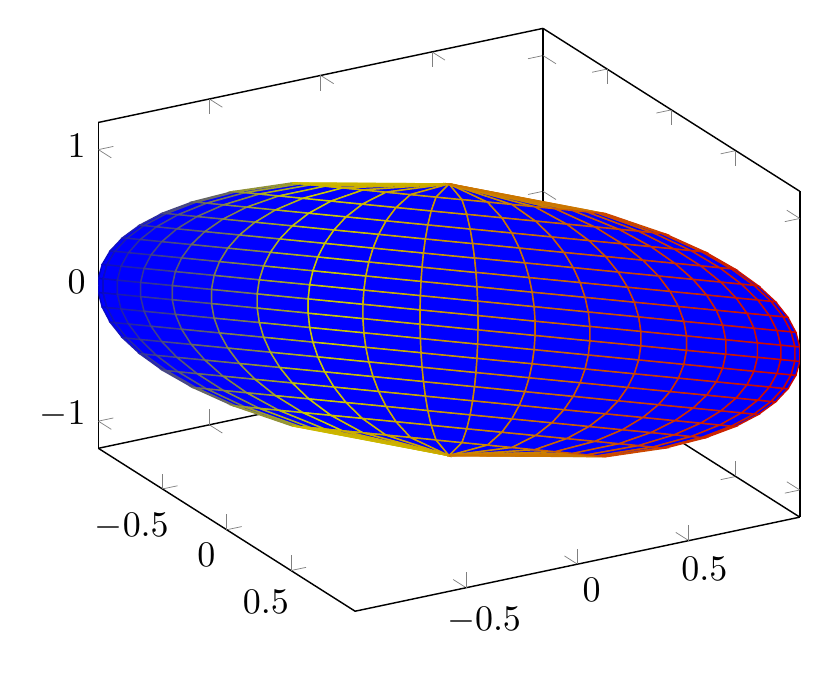
\begin{tikzpicture}[scale=1.3]
    \begin{axis}[samples=20,domain=-1:1,y domain=0:2*pi,view={60}{30}]
      \addplot3 [surf,fill=blue,point meta=x, z buffer=sort] (
        {sqrt(1-x^2)*cos(deg(y)/2)},
        {sqrt(1-x^2)*cos(deg(y)/2)},
        x
        );
    \end{axis}
  \end{tikzpicture}
\end{center}
Questo solido non è uno di quelli il cui volume è immediato, però possiamo immaginare di 
suddividerlo in tante superifici perpendicolare ad un asse. Conoscendo l'area di questa
superficie $S(x)$, il volume del solido diventa semplicemente
\begin{equation*}
  V = \int\limits_{a}^{b} S(x)\,\dif x
\end{equation*}
Si tenga conto che, in una piramide o in un cono, definita $B$ la base, $S$ una superficie 
parallela alla base, $h$ l'altezza del solido e $h'$ la distanza tra la punta e la superifice $S$,
si ha che
\begin{equation*}
  B:S=h^2:h'^2
\end{equation*}

\subsubsection{Lunghezza di un arco di curva}
Data una funzione $f(x)$ il cui grafico può essere
\begin{center}
  \begin{tikzpicture}
    \begin{axis}[xmin=-1,ymin=-1,xmax=4,ymax=3]
      \coordinate (O) at (0,0);
      \node[fill=white,circle,inner sep=0pt] (O-label) at ($(O)+(-135:10pt)$) {$O$};
      \addplot[domain=-1:4,blue,thick] {((cos(deg(x)))/x)*sin(deg(x))+1};
    \end{axis}
  \end{tikzpicture}
\end{center}
In un intorno ${[a,b]}$, la lunghezza di quell'arco di curva è pari a
\begin{equation*}
  l = \int\limits_{a}^{b} \sqrt{1+f'(x)}\,\dif x
\end{equation*}
